\documentclass{article} % For LaTeX2e

%STANDARD PREAMBLE
%https://tex.stackexchange.com/questions/68821/is-it-possible-to-create-a-latex-preamble-header
\usepackage{/Users/mwojno01/Research/Learning/latex_preamble/preamble}

%%% 
% SPECIFIC TO THIS DOCUMENT
%%%

% SIGMA-FIELDS 
% Sigma fields (text)
\renewcommand{\sf}{$\sigma$-field}
\newcommand{\sfs}{$\sigma$-fields}


% SET FUNCTIONS 
%Finitely additive set functions
\newcommand{\fasf}{\tilde{\mu}_0}
% Signed measure
\newcommand{\signedmu}{\wt{\mu}}


% ENUMERATE BUT WITH LETTERS
\newenvironment{alphabate}
    {\begin{enumerate}[label=\alph*)]}
	{\end{enumerate} }
    
\begin{document}


\title{Notes on Probability and Measure Theory} 
\maketitle
\tableofcontents
\newpage 

\section{Overview}

\subsection{References}
The primary reference here is \cite{ash2000probability}.   Unless otherwise specified, all references to the ``text" refers to this textbook.  Likewise the symbol $\S$ refers to a Section of that textbook.

\subsection{Motivation} \label{sec:motivation}

Measure theory serves as a critical underpinning for some of the most interesting research in Bayesian statistics and probabilistic machine learning (see work from Stephen G. Walker, Michael Jordan, Tamara Broderick, David Dunson, and so on).   Thus, fluency with measure theory opens doors to a higher level of research consumption. 
  
It is convenient in unifying various kinds of random variables.  In particular, it allows one to work with discrete and absolutely continuous random variables in a unified way.  For example, the exponential family includes both types of random variables.

Finally, measure theory is important to have a deeper level of understanding of probabilistic concepts.  Probability measures, and measures more generally, cannot be defined on all subsets of many spaces that we would like to deal with.  For instance, non-measurable sets can be shown to exist even for the uniform distribution.  Proposition 1.2.6 of \cite{rosenthal2006first} shows that there is no definition of $P(A)$ that is defined for all subsets $A \subseteq [0,1]$ satisfying all three conditions below
\begin{enumerate}
\item $P([a,b]) = b-a, \quad 0 \leq a \leq b \leq 1$.	
\item $P(\bigcupdot_{n=1}^\infty A_n ) = \ds\sum_{n=1}^\infty A_n$ for $A_1, A_2, ...$ disjoint subsets of $[0,1]$.
\item $P(A \bigoplus r) = P(A), \quad 0 \leq r \leq 1$, where $A \bigoplus r$ denotes the \textit{r-shift} of $A$, i.e. 
\[ A \bigoplus r := \set{a+r : a \in A, a+r \leq 1} \cup \set{a+r-1 : a \in A, a +r >1}\]
\end{enumerate}

The solution to this problem is to define $P$ on a restricted domain, $\sigma$-fields.

%We begin with a discussion of $\sigma$-fields, which are the domains of probability measures, and measures more generally.  As it turns out, measures cannot be defined on all subsets of many spaces that we would like to deal with. For instance, consider Proposition 1.2.6 of \cite{rosenthal2006first} which asserts the existence of non-measurable sets for the uniform distribution.  In particular, there is no definition of $P(A)$ that is defined for all subsets $A \subseteq [0,1]$ satisfying all three conditions below



\section{$\S$ 1.1: Some notes on set theory}

\subsection{Limits of sequences of sets}

\begin{definition}
The \textbf{upper limit} of a sequence of sets is given by
\[ \lim\sup A_n := \bigcap_{n=1}^\infty \bigcup_{k \geq n} A_k \]
Alternatively,
\[ x \in \lim\sup A_n \text{ iff } x \in A_n \text{ for infinitely many } n \]
\end{definition}

\begin{definition}
The \textbf{lower limit} of a sequence of sets is given by
\[ \lim\inf A_n := \bigcup_{n=1}^\infty \bigcap_{k \geq n} A_k \]
Alternatively,
\[ x \in \lim\inf A_n \text{ iff } x \in A_n \text{ eventually ( for all but finitely many $n$ ) } \]
\end{definition}

\begin{figure}
\centering 
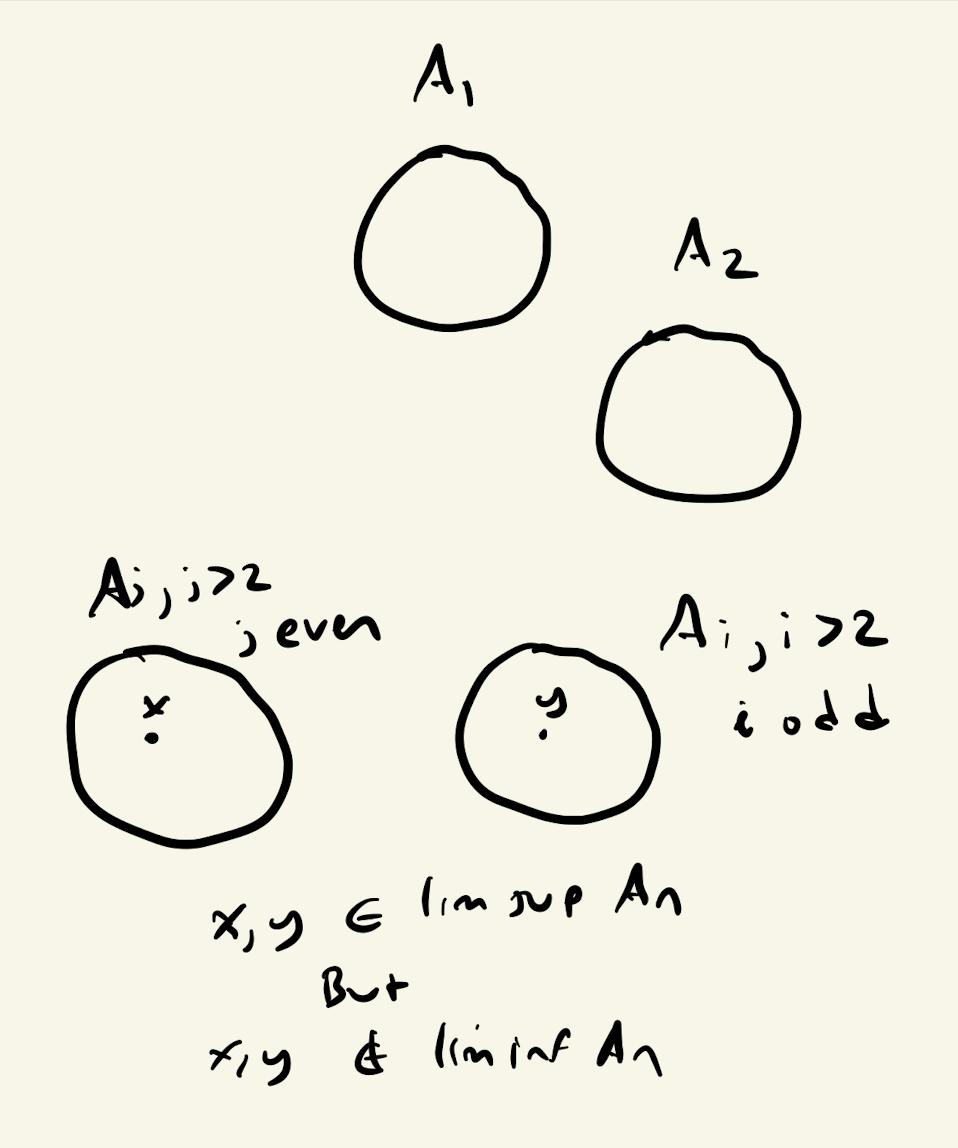
\includegraphics[width=.5\textwidth]{images/limsup_and_liminf}	
\caption{A sequence of sets with empty lower limit and non-empty upper limit.}
\end{figure}

\begin{definition}
If $\lim\inf A_n = \lim\sup A_n = A$, then A is called the \textbf{limit} of the sequence $A_1, A_2, ...$. 
\end{definition}

Now we present a particular kind of limit that will be useful when we discuss continuity of measure. 

\begin{definition}
If $A_1 \subset A_2 \subset ...$ and $\cup_{n=1}^\infty A_n = A$, we say that the $A_n$ form a \textbf{increasing} sequence of sets with limit $A$ or that the $A_n$ increase to $A$; we write $A_n \uparrow A$.  If $A_1 \supset A_2 \supset ... $ and  	$\cap_{n=1}^\infty A_n = A$, we say that the $A_n$ form a \textbf{decreasing} sequence of sets with limit $A$ or that the $A_n$ decrease to $A$; we write $A_n \downarrow A$.
\end{definition}


\begin{figure}
\centering 
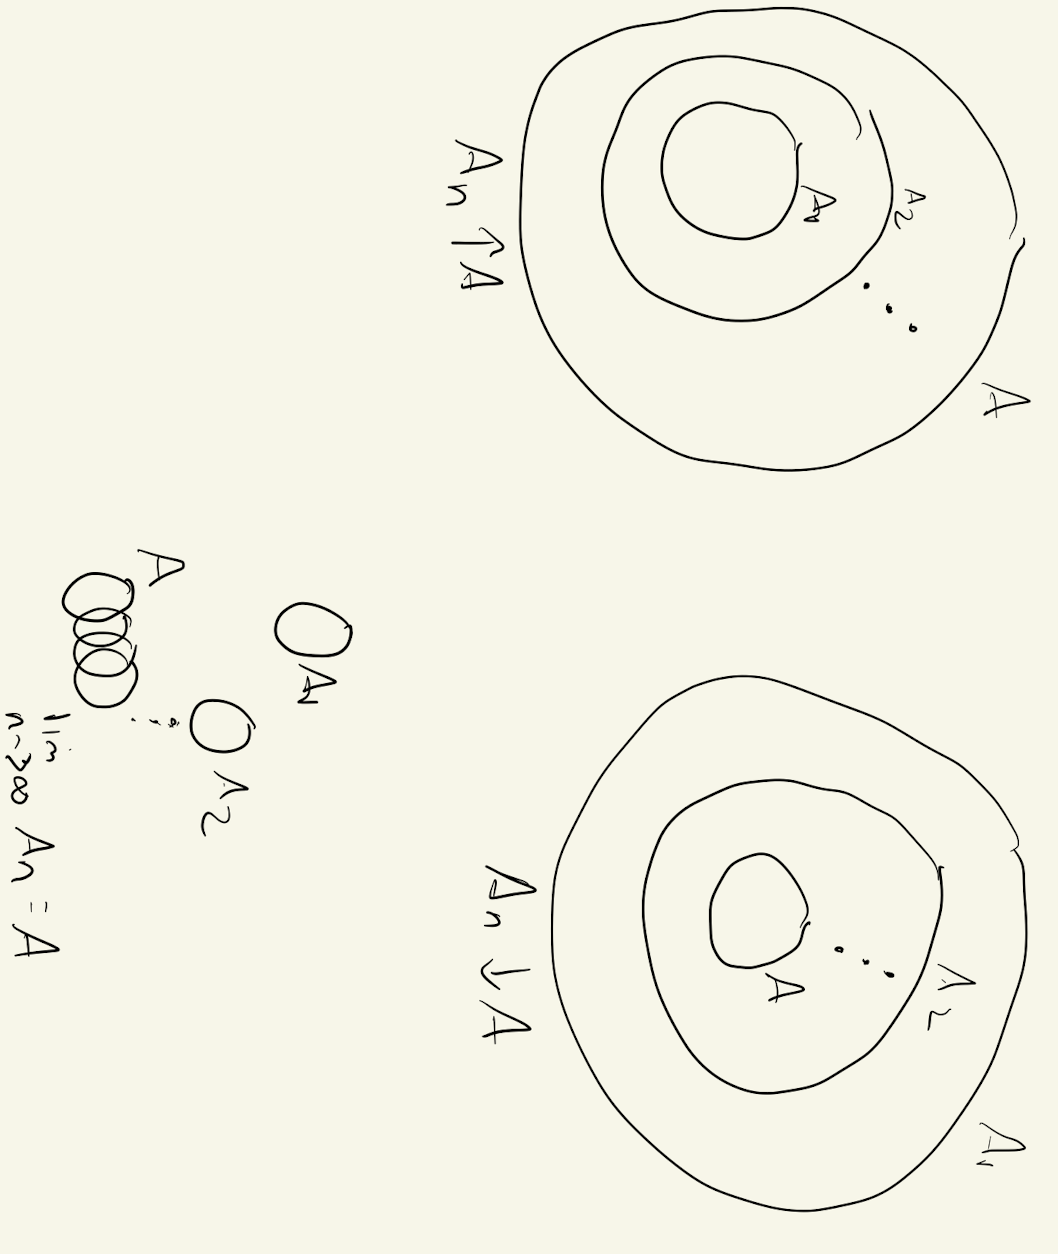
\includegraphics[width=.5\textwidth, angle=90]{images/increasing_and_decreasing_sequences}
\caption{An increasing and decreasing sequence of sets, followed by a sequence of sets which is neither, but which has a limit.}
\end{figure}

One can verify that this definition is consistent with the definition of limits, i.e.
\[  \text{If } A_n \uparrow A \text{ or } A_n \downarrow A \text{ then } \lim\inf A_n = \lim\sup A_n = A.\]

\subsection{Representing unions as disjoint unions}
 
\begin{remark}
If $A_1,A_2,...$ are subsets of some set $\Omega$, then
\begin{align*} 
\bigcup_{n=1}^\infty A_n = \bigcupdot_{n=1}^\infty \bigg(A_n \cap A_{n-1}^c \cap ... \cap A_1^c \bigg) 	
\labelit \label{eqn:union_as_disjoint_union}
\end{align*}

In other words, any union can be re-represented as a disjoint union. This is useful because measures are countably additive on disjoint sets, so we prefer to work with collections of disjoint sets.
\label{rk:rerepresenting_unions_as_disjoint_unions}
\end{remark}

\begin{remark}
If $A_n \uparrow A$, then \eqref{eqn:union_as_disjoint_union} becomes
\begin{align*}
	\bigcup_{n=1}^\infty A_n = \bigcupdot_{n=1}^\infty \bigg( A_n - A_{n-1} \bigg) 
\labelit \label{eqn:union_as_disjoint_union_for_increasing_sequences}
\end{align*}
This is because $A_{n-1} \subset A_{n}$, so $A_{n-1}^c \supset A_{n}^c$ by contraposition.	
\end{remark}

\section{$\S$ 1.2: Fields, \sfs, measures}

\subsection{$\S$ 1.2.1-1.2.2: Fields and \sfs}

\subsubsection{$\sigma$-fields}

We begin with a discussion of $\sigma$-fields, which are the domains of probability measures, and measures more generally.  As stated in the motivation (Section \ref{sec:motivation}), measures cannot be defined on all subsets of many spaces that we would like to deal with. 

%\sfs\ are important because they are the domain of measures.  
%Here are some definitions.

\begin{definition}
Let $\F$ be a collection of subsets of a set $\Omega$.  Then $\F$ is called a \textbf{sigma-field} (or \textit{sigma-algebra}) if it satisfies

\begin{enumerate}[label=\alph*)]
	\item $\Omega \in \F$ 
	\item If $A \in \F$, then $A^c \in \F$.
	\item If $A_1,A_2, ... \in \F$ then $\cup_{i=1}^\infty A_i \in \F$.  
\end{enumerate}
that is, if $\Omega \in \F$ and $\F$ is closed under complementation and finite unions.
\label{def:sigma_field}	
\end{definition}

\begin{example}
$\F =\set{\emptyset, \Omega}$ is the smallest \sf\ on $\Omega$. 
\end{example}

\begin{example}
	$\F =2^\Omega$, i.e. the set of all subsets of $\Omega$, is the largest \sf\ on $\Omega$.
\end{example}

\begin{example}
If $A \in \Omega$ is non-empty, then $\F = \set{\emptyset, A, A^c, \Omega}$ is the smallest \sf\ containing $A$.
\end{example}

\begin{notation}
If $\C$ is a class of sets, the smallest \sf\ containing the sets of $\C$ is written as $\sigma(\C$).  This is sometimes called the \textit{minimal \sf\ over $C$} or the \textit{\sf\ generated by $C$}. 
\end{notation}
	
\begin{question}
Let $A_1,...,A_n$ be subsets of $\Omega$.  Describe $\F := \sigma(\set{A_1,...,A_n})$, the smallest \sf\ containing $A_1,...,A_n$.  Also describe the number of sets in $\F$.   \textit{This is Ash's Problem 1.2.8.  We can derive the strict upper bound $|\F| \leq 2^{2^n}$. For a complete answer, see GoodNotes. }	
\end{question}

\subsubsection{Fields}

Fields are more general than $\sigma$-fields.  Measures are sometimes constructed by being defined on fields, and then extended to \sfs.  Indeed, we will see this strategy with Lesbesgue measure. 

\begin{definition}
Let $\F$ be a collection of subsets of a set $\Omega$.  Then $\F$ is called a \textbf{field} (or \textit{algebra})  if satisfies Definition \ref{def:sigma_field} after replacing condition c) with

\begin{enumerate}
	\item[c')] If $A_1,...A_n \in \F$ then $\cup_{i=1}^n A_i \in \F$.
\end{enumerate}
that is, if $\Omega \in \F$ and $\F$ is closed under complementation and \textit{finite} unions.
\label{def:field}	
\end{definition}

\begin{example} What is an example of a collection that is a \textit{field}, but not a $\sigma$-\textit{field}?  

Let $\Omega=\R$ and $\F_0 = \set{\text{finite disjoint unions of right semi-closed intervals } (a,b], a \neq b}$.  Then $\F_0$ is a field, as can be easily verified.\footnote{By convention, we also count $(a, \infty)$ as right semi-closed for $-\infty\leq a < \infty$, which is necessary for the \sf\ to be closed under complements.}   

\begin{figure}[h!]
\centering
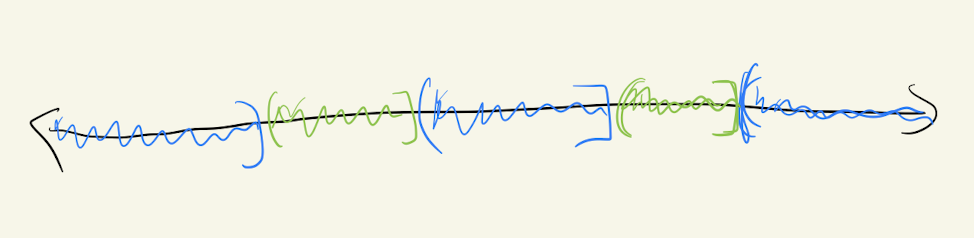
\includegraphics[width=.6\textwidth]{images/rsc_intervals}	
\end{figure}

But $\F_0$ is \underline{not} a \sf.  Note that if $A_n = (-\frac{1}{n},0]$, then $\bigcap_{n=1}^\infty A_n = \set{0}  \not\in \F_0$.
\label{ex:field_of_finite_disjoint_unions_of_lsc_intervals}
\end{example}

\begin{remark}
A \sf\ can also be described as a field that is closed under limits of increasing sequences.  For if $A_n \in \F$ and $A_n \uparrow A$, then A is a countable union of sets in $\F$ by definition.  Conversely, if $A = \cup_{n=1}^\infty A_n$, then set $B_N := \cup_{n=1}^N A_n$ and $B_N \uparrow A$.	
\end{remark}


\subsubsection{``Good sets" strategy}

Ash says that there is a type of reasoning that occurs so often in problems involving \sfs that it deserves explicit mention.  It is called the \textit{good sets strategy}.   Suppose you want to show that all members of a $\sigma$-algebra   $\F$ have some property $P$.  Define ``good sets" as those that satisfy the property
\[ \G := \{ G \in \F : G \text{ has property } P \} \]
The strategy is then to simply
\begin{enumerate}
\item Show $\G$ is a $\sigma$-algebra 
\item Show $\G$ contains some class $\C$ such that $\F = \sigma(\C)$	
\end{enumerate}


Then you're done!  

Why does this work?

\begin{align*}
& \quad \C \subset \G &&	\text{by 2}\\
&\implies \sigma(\C) \subset \sigma(\G) &&  \\
&\implies \F \subset \G && \text{by 1,2} \\
& \text{Yet $\G \subset \F$ by definition of $\G$.} && \\
& \text{So $\G = \F$.} && \\
& \text{ So all sets in $\F$ are good.} && \\
\end{align*}

In the text, Ash uses this strategy to show that if $\C$ is a class of subsets of $\Omega$, and $A \in \Omega$, then

\[ \explaintermbrace{take minimal sigma field first, then intersect}{\sigma_\Omega(\C) \cap A} = \explaintermbrace{intersect first, then take minimal sigma-field}{\sigma_A(\C \cap A)} \]

 For another application, see handwritten homework exercises.	

\subsection{$\S$ 1.2.3-1.2.4: Measures}




\begin{definition}
A \textbf{measure} on a \sf\ $\F$ is a non-negative, extended real-valued function $\mu$ on $\F$ such that whenever $A_1, A_2, ...$ form a finite or countably infinite collection of disjoint sets in $\F$, we have countable additivity; that is,
\[ \mu \bigg( \bigcupdot_n A_n \bigg) = \ds\sum_n \mu(A_n) \]
\label{def:measure}	
\end{definition}

\begin{definition}
A \textbf{probability measure} is a measure (Definition \ref{def:measure}) where $\mu(\Omega)=1$.
\label{def:prob_measure}		
\end{definition}

\begin{remark}
Ash additionally assumes that a measure does not take $\mu(A) = \infty$ or $\mu(A) = -\infty$ for all $A \in \F$.  From this, we automatically obtain $\mu(\emptyset)=0$. For $\mu(A) < \infty$ for some $A$, and by considering the sequence $A, \emptyset, \emptyset, ...$, we have that $\mu(\emptyset)=0$ by countable additivity.   	
\end{remark}

\begin{example}
Let $\Omega = \set{x_1,x_2,...}$ be a finite or countably infinite set.  Let $p_1, p_2,...$ be non-negative reals.  Let $\F = 2^\Omega$.  Define
\[\mu(A) = \ds\sum_{x_i \in A} p_i \quad \text{ for all } A \in \F\]
Then $\mu$ is a measure on $\F$. We might call it the ``point weighting" measure. 
\begin{itemize}
\item If $p_i \equiv 1 \; \forall \, i$, then $\mu$ is called the \textbf{counting measure}.
\item If $\sum_i p_i =1$, then $\mu$ is a probability measure.	
\end{itemize}
	
\end{example}


\begin{example}{\remarktitle{Lesbesgue measure}}
Define $\mu$ such that 
\[ \mu(a,b] = b-a \quad \forall \, a,b \in \R : b>a \]
As we will see in Section \ref{sec:extension_of_measures}, this requirement determines $\mu$ on a large collection of sets, the Borel Sets $\B(\R)$, defined as the smallest \sf\ of subsets of $\R$ containing all intervals $(a,b] \subset \R$.

We may alternately characterize $\B(\R)$ as the smallest \sf\ containing
\begin{itemize}
\item all intervals $[a,b], \; a,b \in \R$.
\item all intervals $(a,b), \; a,b \in \R$
\item all intervals $(a,\infty), \; a \in \R$.
\item  all intervals $[a,\infty), \; a \in \R$.
\item 	 all intervals $(-\infty,b), \; b \in \R$.
\item  all intervals $(-\infty,b], \; b \in \R$.
\item  all intervals $[a,b], \; a,b \in \R$.
\item all open sets of $\R$.\footnote{Recall that an open set is a countable union of open intervals.}
\item all closed sets of $\R$.\footnote{Recall that a set is open iff its complement is closed.}
\end{itemize}

To illustrate these equivalences, let us equate the first two conditions. That is, let us show that a \sf\ contains all open intervals $(a,b)$ iff it contains all right semi-closed intervals $(a,b]$.  To see this, simply note

\begin{align*}
(a,b] &= \bigcap_{n=1}^\infty \bigg(a, b+\frac{1}{n}\bigg) \\
	\intertext{and}
(a,b) &= \bigcup_{n=1}^\infty \bigg(a, b-\frac{1}{n}\bigg] 
\end{align*}

\end{example}

\begin{question}
The text gives another description of the Borel sets $\B(\R)$ as the smallest \sf\ containing $\F_0$, the field of disjoint unions of right semi-closed intervals $(a,b]$.  Can we make the same statement about the field of finite disjoint unions of left semi-closed intervals?
\end{question}

\subsection{$\S$ 1.2.5-1.2.6: Measure-like set functions, and their properties}

The text considers some generalizations of measures that can be obtained by restricting the domain to a field, by assuming merely finite additivity, or by allowing the range to be extended reals ($\bar{\R}$) instead of non-negative extended reals ($\bar{\R}_{\geq 0}$).  

\begin{remark}
The first two relaxations above often go together.
However, a  countably additive function can be defined on a \textit{field} (rather than \sf) if the condition is taken to hold whenever a countable union \textit{does} happen to still be in the field.  In my notes, I will simply things by assuming that countably additive functions are always defined on \sfs.
\label{rk:i_am_assuming_a_domain_based_on_the_type_of_additivity}
\end{remark}	



\begin{table}[!h]
\centering	
\begin{tabular}{rcc}
&\multicolumn{2}{c}{\textbf{Range}} \\
& \textbf{non-negative} & \textbf{signed} \\
\textbf{finitely additive}& $\mu_0$ & $\tilde{\mu}_0$ \\	
\textbf{countably additive}& $\mu$ measure  & $\tilde{\mu}$ signed measure \\

\end{tabular}
\caption{Notation for generalizations of measure (For assumed domain in each case, see Remark \ref{rk:i_am_assuming_a_domain_based_on_the_type_of_additivity}.)}
\label{tab:notation_for_generalizations_of_measure}
\end{table}

In Table \ref{tab:notation_for_generalizations_of_measure},  we introduce some notation to try to clarify more immediately when results hold. Note the relations\footnote{So, for example, if something holds for $\tilde{\mu}_0$, it holds for $\mu$.  A simple mnemonic is that adding stuff to the notation generalizes the function.}  
\[ \set{\mu} \subset \set{\mu_0}, \set{\tilde{\mu}} \subset \set{\tilde{\mu}_0}. \]
 
 \begin{example} Let $\F_0$ be the field of finite disjoint unions of right semi-closed intervals (see Definition \ref{def:rsc_intervals} ), and define the set function $\fasf$ on $\F_0$ as follows\footnote{This example comes from Problem 4 in Section 1.2 of the text}:

\begin{align*}
\fasf(-\infty,a] &=a, && a \in \R  \\
\fasf(a,b] &= b-a, && a,b \in \R, \quad a<b  \\
\fasf(b, \infty) &= -b, && b \in \R \\
\fasf(\R) &=0 &&\\
\fasf(\bigcupdot_{i=1}^n I_i) &= \sum_{i=1}^n \fasf(I_i), && \text{if $I_1, ..., I_n$ are right semi-closed intervals} 
\end{align*}
	
Then $\fasf$ is finitely additive, but not countably additive on $\F_0$.   For a proof, see GoodNotes.
 \end{example}

 
Measure-like set functions have useful properties. Using the notation in Table \ref{tab:notation_for_generalizations_of_measure}, we rewrite Theorem 1.2.5 of the text:
 
 \begin{theorem}
 Let $\fasf$ be a finitely additive set function on the field $\F_0$.  Then
 \begin{enumerate}[label=\alph*)]
 \item \label{itm:first} $\fasf(\emptyset)=0$
 \item \label{itm:second} $\fasf(A \cup B) + \fasf (A \cap B) = \fasf(A) + \fasf(B)$ for all $A,B \in \F_0$.
 \item \label{itm:piece-and-difference} If $A,B \in \F_0$ and $B \subset A$, then   
  \[ \fasf(A) = \fasf(B) + \fasf(A-B)\quad \text{(piece-and-difference)} \] 
 So $\fasf(A) \geq \fasf(B)$ if $\fasf(A-B) \geq 0$. More generally, for non-negative set functions, we have
 \[ \mu_0 (A) \geq \mu_0 (B) \quad \text{(monotonicity)} \] 
 \item \label{itm:subadditivity} Subadditivity holds if $\fasf$ is non-negative, i.e.
 \begin{align*}
 \mu_0 (\cup_{i=1}^n A_i)& \leq \sum_{i=1}^n \mu_0(A_i) \\
  \mu (\cup_{i=1}^\infty A_i)& \leq \sum_{i=1}^\infty \mu(A_i) \\
 \end{align*}
 \end{enumerate}
\label{thm:basic_properties_of_finitely_additive_set_functions}
 \end{theorem}
  
\begin{proof}
 We prove Theorem \ref{thm:basic_properties_of_finitely_additive_set_functions} (b).  The rest is an exercise for the reader (or see the text).
 
 First, we break things into disjoint pieces
 {\footnotesize 
\begin{align*}
A &= \bigg(A \cap B \bigg) \, \bigcupdot \, \bigg(A \cap B^c \bigg)	&& \implies \fasf(A) = \fasf (A \cap B) +  \fasf (A \cap B^c)  && (1) \\
B &= \bigg(A \cap B \bigg) \, \bigcupdot \, \bigg(A^c \cap B \bigg)	&& \implies \fasf(B) = \fasf (A \cap B) +  \fasf (A^c \cap B)  && (2) \\
A \cup B &= \bigg(A \cap B \bigg) \, \bigcupdot \, \bigg(A \cap B^c \bigg) \bigcupdot \, \bigg(A^c \cap B \bigg)	&& \implies \fasf(A \cup B) = \fasf (A \cap B) +  \fasf (A \cap B^c) + \fasf (A^c \cap B)   && (3) 
\end{align*}
}

Summing (1) and (2), we obtain
\[\fasf(A) + \fasf(B) = 2 \fasf(A \cap B) + \fasf(A \cap B^c) + \fasf(A^c \cap B). \]
We use (3) to simplify the RHS, and the result follows.
\end{proof}

\begin{remark}
In the proof of Theorem \ref{thm:basic_properties_of_finitely_additive_set_functions} (b), note that we use a common strategy -- breaking sets into disjoint pieces so that we can apply the assumed (finite or countable) additivity of the set function. 
\end{remark}


\begin{remark}
Is \textit{finiteness} ($|\mu_g (A)| < \infty \; \forall \; A \in \F_g$) equivalent to \textit{boundedness} ($\sup \set{|\mu_g (A)| : A \in \F_g} < \infty$)?
\begin{itemize}
\item $\mu_0, \signedmu$ ? \greencheck
\item $\fasf$ ? \redx (too general)
\end{itemize}
The fact that equivalence holds for signed measures $\signedmu$ is surprising.  Somehow countable additivity compensates for the signedness. See Section 2.1.3 of the text. 
\end{remark}

 
\begin{remark}
Being able to work with these generalizations will be important in Section \ref{sec:extension_of_measures} on extension of measures.  In particular, it will help us show that we can construct the Lesbesgue measure on the Borel sets.
\end{remark}

\subsection{$\S$ 1.2.7-1.2.8: Continuity of countably additive set functions}

Countably additive set functions have a basic continuity property. Continuity of measure is a special case. 

\begin{theorem}
Let $\signedmu$ be a countably additive set function on the \sf\ $\F$. Then

\begin{alphabate}
\item (continuity from below) If $A_1, A_2, ... \in \F$ and $A_n \uparrow A$, then $\signedmu(A_n) \to \signedmu(A)$ as $n \to \infty$. 
\item (continuity from above)  If $A_1, A_2, ... \in \F$, $A_n \downarrow A$, and $\signedmu(A_n)$ is finite, then $\signedmu(A_n) \to \signedmu(A)$ as $n \to \infty$. 
\end{alphabate}
\label{thm:continuity_of_countably_additive_set_functions}
\end{theorem}

\begin{proof}
We prove continuity from below, and leave continuity from above as an exercise to the reader (or see text).  First let us assume that all $\signedmu(A_n)$ are finite (*). Then 
\begin{align*}
A &= A_1 \cupdot A_2 - A_1 \cupdot A_3 - A_2 \cupdot ... && 	\text{ by } \eqref{eqn:union_as_disjoint_union_for_increasing_sequences} \\
\implies \signedmu(A) &= \signedmu(A_1) + \signedmu(A_2 - A_1) + \signedmu(A_3 - A_2) + ... && \text{(countable additivity)}\\ 
&= \signedmu(A_1) + \signedmu(A_2) - \signedmu(A_1) + \signedmu(A_3) - \signedmu(A_2) + ... && \text{(Theorem \ref{thm:basic_properties_of_finitely_additive_set_functions} \ref{itm:piece-and-difference}, (*) }\\
&= \ds\lim_{n \to \infty} \signedmu(A_n) 
\end{align*}
Now suppose $\signedmu(A_n) = \infty$ for some $n$.   So write 
\begin{align*}
A &= A_n \cupdot A- A_n && \text{(increasing sequence)}\\ 
\implies \signedmu(A) &= \signedmu(A_n) + \signedmu(A - A_n) && \text{(countable additivity)}\\  
&= \infty + \signedmu(A - A_n) 
\end{align*}

So $\signedmu(A)=\infty$.\footnote{Note that we cannot have $\signedmu(A - A_n)=-\infty$, because that would violate additivity.} Replace $A$ by $A_k$ for any $k \geq n$ to also find $\signedmu(A_k)=\infty$ for all $k \geq n$ and the result follows.

Finally suppose $\signedmu(A_n) = -\infty$ for some $n$. Then the result follows in the same way as for $\signedmu(A_n) = \infty$. 

\end{proof}

\begin{remark}
The logic of the proof of Theorem \ref{thm:continuity_of_countably_additive_set_functions} under the finiteness assumption is as follows.  First, we re-represent the union as a disjoint union (the form is particularly simple since the sets are increasing).  This allows us to apply countable additivity. Then we apply the piece-and-difference decomposition (and the subtraction is defined under the finiteness assumption). 	
\end{remark}

\begin{remark}
In proving Theorem \ref{thm:continuity_of_countably_additive_set_functions}  for the case where $\mu(A_n) = \infty$ for some $n$, it is tempting to make the simpler argument 
\begin{align*}
\mu(A) & \geq \mu(A_n) && \text{(monotonicity)}\\	
\mu(A_k) & \geq \mu(A_n) && \text{(monotonicity)}	 
\end{align*}
for $k \geq n$.  But recall from Theorem \ref{thm:basic_properties_of_finitely_additive_set_functions} that monotonicity only holds under non-negativity, and the theorem statement is more general, applying to \textit{signed} set functions as well. 
\end{remark}

We have the result that finite additivity plus continuity equals countable additivity. 

\begin{theorem}
Let $\fasf$ be a finitely additive set function on the field $\F_0$.  Then $\fasf$ is countably additive if either
\begin{alphabate}
\item $\fasf$ is continuous from below
\item $\fasf$ is continuous from above at the empty set.	
\end{alphabate}

\begin{proof}
We prove (a) and leave (b) as an exercise to the reader (or see text). 	%To show that $\fasf$ is countably additive, we need to show that  $ \fasf \bigg( \bigcupdot_{n=1}^\infty A_n \bigg) = \ds\sum_{n=1}^\infty \fasf(A_n)$.   

Given $A = \bigcupdot_{n=1}^\infty A_n$, we define $P_n := \bigcup_{m \leq n} A_n$ and so $P_n \uparrow A$.   So we have
\begin{align*}
\fasf(P_n) &\to \fasf(A) && \text{(continuity from below)} \\
\implies \fasf(\bigcup_{m \leq n} A_n) &\to \fasf(A) && \text{(definition)} \\	
\implies \ds\sum_{m=1}^n \fasf(A_n) &\to \fasf(A) && \text{(finite additivity)} \\
\end{align*}
Taking $n \to \infty$ gives countable additivity.
\end{proof}

\end{theorem}



%By , we have


 %we break up the limit of the increasing sequence into a disjoint union as follows	



 \section{$\S$ 1.3: Extension of measures} \label{sec:extension_of_measures}
 

\bibliography{references_ash_notes.bib}
\bibliographystyle{unsrt}

\appendix

\section{Definitions}

\begin{definition}
A \textbf{right semi-closed interval} is a set of the form $(a,b] = \set{x : a < x \leq b}, -\infty \leq a < b < \infty$.  By convention, we also count $(a,\infty)$ as right semi-closed for $-\infty \leq a < \infty$. 
\label{def:rsc_intervals}
\end{definition}



\end{document}
